\documentclass[a4paper]{article}

% --- Packages ---

\usepackage{a4wide}
\usepackage[utf8]{inputenc}
\usepackage{amsmath}
\usepackage{mathtools}
\usepackage{amssymb}
\usepackage[english]{babel}
\usepackage{mdframed}
\usepackage{systeme,}
\usepackage{lipsum}
\usepackage{relsize}
\usepackage{caption}
\usepackage{tikz}
\usepackage{tikz-3dplot}
\usetikzlibrary{shapes.geometric}
\usepackage{pgfplots}
\usepackage{pgfplotstable}
\pgfplotsset{compat=newest}%1.7}
\usepackage{harpoon}%
\usepackage{graphicx}
\usepackage{wrapfig}
\usepackage{subcaption}
\usepackage{authblk}
\usepackage{float}
\usepackage{listings}
\usepackage{xcolor}
\usepackage{chngcntr}
\usepackage{amsthm}
\usepackage{comment}
\usepackage{commath}
\usepackage{hyperref}%Might remove, adds link to each reference
\usepackage{url}
\usepackage{calligra}
\usepackage{pgf}

% --- Bibtex ---
% To run our bibliography, we need to compile the ref document
% `biber main` or `biber ref` in the terminal
% We can compile the document with `pdflatex main` or `latex main`

\usepackage{csquotes}
\usepackage[
    %backend=biber,
    backend = biber,
    style=phys,
    sorting=ynt,
]{biblatex}

%\addbibresource{ref.bib}


% --- Commands --- 

\newcommand{\w}{\omega}
\newcommand{\trace}{\text{Tr}}
\newcommand{\grad}{\mathbf{\nabla}}
%\newcommand{\crr}{\mathfrak{r}}
\newcommand{\laplace}{\nabla^2}
\newcommand{\newparagraph}{\vspace{.5cm}\noindent}

% --- Math character commands ---

\newcommand{\curl}[1]{\mathbf{\nabla}\times \mathbf{#1}}
\newcommand{\dive}[1]{\mathbf{\nabla}\cdot \mathbf{#1}}
\newcommand{\res}[2]{\text{Res}(#1,#2)}
\newcommand{\fpartial}[2]{\frac{\partial #1}{\partial #2}}
\newcommand{\rot}[3]{\begin{vmatrix}\hat{x}&\hat{y}&\hat{z}\\\partial_x&\partial_y&\partial_z\\#1&#2&#3 \end{vmatrix}}
\newcommand{\average}[1]{\langle #1 \rangle}
\newcommand{\ket}[1]{|#1\rangle}
\newcommand{\bra}[1]{\langle #1|}


%  --- Special character commands ---

\DeclareMathAlphabet{\mathcalligra}{T1}{calligra}{m}{n}
\DeclareFontShape{T1}{calligra}{m}{n}{<->s*[2.2]callig15}{}
\newcommand{\crr}{\mathcalligra{r}\,}
\newcommand{\boldscriptr}{\pmb{\mathcalligra{r}}\,}


\title{INPUT TITLE HERE}
\author{Author : Andreas Evensen}
\date{Date: \today}

% --- Code ---

\definecolor{codegreen}{rgb}{0,0.6,0}
\definecolor{codegray}{rgb}{0.5,0.5,0.5}
\definecolor{codepurple}{rgb}{0.58,0,0.82}
\definecolor{backcolour}{rgb}{0.95,0.95,0.92}

\lstdefinestyle{mystyle}{
    backgroundcolor=\color{backcolour},   
    commentstyle=\color{codegreen},
    keywordstyle=\color{magenta},
    numberstyle=\tiny\color{codegray},
    stringstyle=\color{codepurple},
    basicstyle=\ttfamily\footnotesize,
    breakatwhitespace=false,         
    breaklines=true,                 
    captionpos=b,                    
    keepspaces=true,                 
    numbers=left,                    
    numbersep=5pt,                  
    showspaces=false,                
    showstringspaces=false,
    showtabs=false,                  
    tabsize=2
}

\lstset{style=mystyle}

\begin{document}
\begin{titlepage}
    \begin{center}
        \vspace*{1cm}
        
        \Huge
        \textbf{Variational Monte Carlo}
        
        \vspace{0.5cm}
        \LARGE
        FK8029 - Computational Physics
        
        \vspace{1.5cm}
        
        \textbf{Andreas Evensen}
        
        \vfill
        
        %\includegraphics[width=0.4\textwidth]{UiO_Segl_pantone.eps}
        
        \Large
        Department of Physics\\
        Stockholm University\\
        Sweden\\
        \today
    \end{center}
\end{titlepage}

%\maketitle

\section{Introduction}
In the last report, we solved the time indepedent Schrödinger equation using two methods, in order to obtain the eigen-states of the system?
This method works for larger systems too, however, the computational cost increases drastically with the number of particles.
Hence, certain methods have been developed in order to solve such equations with less computational cost. One such way is the use of variational Monte Carlo.

\newparagraph
In this report, we solve the time independent Schrödinger equation for the harmonic oscillator using the variational Monte Carlo method.
Furthermore, to see the potential of the method, we also solve the system for a more complex system -- quantum dots.

\tableofcontents

\newpage

\section{Theory \& Method}
The time independent Schrödinger equation is given by:
\begin{align*}
    \hat{H}\ket{\psi} = E\ket{\psi},
\end{align*}where $\ket{\psi}$ is the state of the system, in this case, the wave-function.
The Hamiltonian $\hat{H}$ is system specific, and since we're solving for two systems, we have two different Hamiltonians.
In the first case, we use the Harmonic oscillator, where the Hamiltonian is given by, in reduced units:
\begin{align}
    \hat{H} = -\frac{1}{2}\frac{d}{dz} + \frac{1}{2}z^2,\label{eq: harmonic_oscillator Hamiltonian} 
\end{align}and in the second case, we investigate quantum dots, with the following Hamiltonian, again in reduced units:
\begin{align}
    \hat{H} = \left(\sum_{i = 1}^2 -\laplace_i + \abs{\mathbf{x}_i}^2\right) + \frac{\lambda}{\sqrt{(x_1 - x_2)^2 + (y_1 - y_2)^2}}.\label{eq: quantum dots Hamiltonian}
\end{align}In the above definition, $\mathbf{x}_i = (x_i, y_i)$ is the position of particle $i$, and $x_i$ and $y_i$ are the coordinates of the particle.
The above Hamiltonian is for two particles, and the sum over the contribution both particles feel from a potential well.
The second term is a coupling factor, which couples the two particles to an electromagnetic field.
From this, we define the local energy, $E_{loc}$, to be the energy obtained by the wave-function at a specific location instead of the entire domain. This is then written as:
\begin{align*}
    E_{loc} = \frac{\hat{H}\psi_T}{\psi_T}.
\end{align*}Here $\psi_T$ is the trail wave-function evaluated at a specific point.
This however, implies that the trail wave-function is the true wave-function.
Therefore, we introduce the variational principle, which states that we which minimize the local energy of the system, in order to find the ground state.
We do this by a parameter $\alpha$, which we vary in order to find the minimum energy of the system.
\begin{align}
    E_{loc}^\alpha = \frac{\hat{H}\psi_T^\alpha}{\psi_T^\alpha}. \label{eq: local energy minimize}
\end{align}Thus, we solve for the ground state of the system by minimizing the local energy, $E_{loc}$, with respect to $\alpha$.

\newparagraph
Monte Carlo methods build upon the idea of random sampling, with some probability weighting.
The metropolis algorithm includes a random walk, where every state in the system is reachable from any other state, from a condition called detailed balance.
The algorithm is as follows:
\begin{enumerate}
    \item Pick a random atom
    \item Propose a move
    \item Calculate the probability of the move, $p$ 
    \item Accept or reject the move depending on $\min\left(1, p\right)$
    \item Update the system (if move was accepted, otherwise keep the system as it was).
\end{enumerate}These steps are then repeated for a number of iterations, until the system has reached equilibrium, e.g. when the system is erigodic.
Furthermore, we also sample the systems observables, such as the energy, in order to calculate the expectation value of the system, as well as its variance.
The probability of the move, $p$ is given by the ratio of the probabilities of the trail wave-functions, $\psi_T$:
\begin{align}
    p = \abs{\frac{\psi_T^\alpha(\mathbf{X}')}{\psi_T^{\alpha}(\mathbf{X})}}^2,\label{eq: probability of move}
\end{align}where $\mathbf{X}'$ is the new configuration, and $\mathbf{X}$ is the old configuration.

\newparagraph
In order to minimize the local energy, we could use various methods, such as golden search or steepest descent.
In this report, we use golden search which is a method that finds the minimum of domain given four points. Suppose we have a potential given by the figure below, fig \ref{fig: golden search}.
If we define two points $a$ and $d$, where there exists a single local minimum in the interval $[a, d]$, then we can define two points $a$ and $d$, which constitute a subinterval $[b,c]$ in $[a,d]$.
Then we compute the value as then we compute the value $f(b)$ and $f(c)$, and if $f(b) < f(c)$, then we set $d = c$, otherwise we set $a = b$.
We continue doing this until the difference between $b$ and $c$ is small enough such that we have found the point of the minima.
\begin{figure}[H]
    \centering
    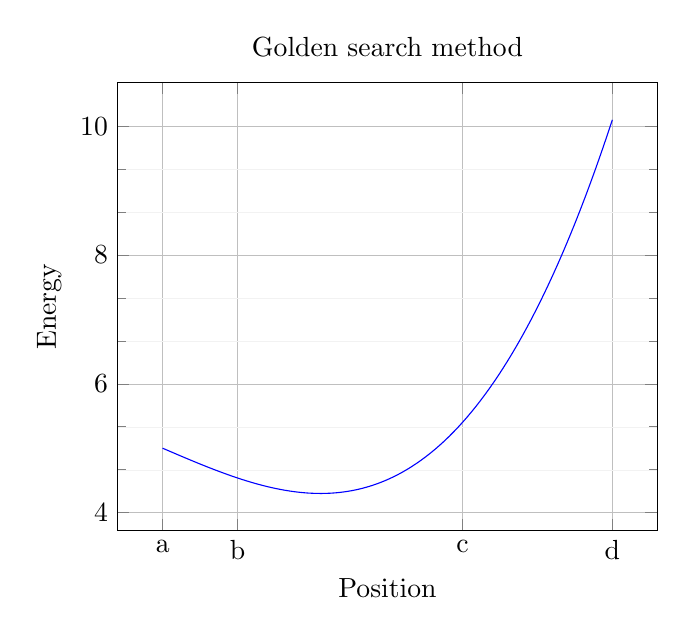
\begin{tikzpicture}
        \begin{axis}[xlabel = {Position}, ylabel = {Energy}, title = {Golden search method},
            grid = both,
            grid style={line width=.1pt, draw=gray!10},
            major grid style={line width=.2pt,draw=gray!50},
            minor tick num=2,
            xtick = {0, 0.5, 2, 3},
            xticklabels = {a, b, c, d},
            ]
            \addplot[domain = 0:3, samples = 100, color = blue]{(0.3 * x^2 - 1) * x + 5};
        \end{axis}
    \end{tikzpicture}
    \caption{Visualisation of the golden search method.}
    \label{fig: golden search}
\end{figure}\noindent
We use this method to find the local minimum of the observables in the system, where we minimize the free parameter $\alpha$, defined in eq \eqref{eq: local energy minimize}
The observables, $\average{E}$ and $\sigma(E)$, are then calculated by the following equations:
\begin{align}
    \average{E} &= \frac{1}{N}\sum_{i = 1}^N E_{loc}^\alpha, \label{eq: average energy}\\
    \sigma(E) &= \left(\frac{1}{N}\sum_{i = 1}^N \left(E_{loc}^\alpha\right)^2 - \average{E}^2\right)^{\frac{1}{2}},\label{eq: variance energy}
\end{align}where $N$ is the number of samples taken.
\newpage
\section{Result \& Discussion}
This section is dedicated to the presentation of the results obtained from the variational Monte Carlo simulation, and a discussion of the results.
Moreover, the results were obtained simulation written in \verb|V|.

\subsection{Harmonic Oscillator}
In this section, we present the results of the variational Monte Carlo method for the harmonic oscillator case, eq \ref{eq: harmonic_oscillator Hamiltonian}, in a one-dimensional potential.
The ground state of a harmonic oscillator is known to be a Gaussian, and thus we provide the following trail wave-function:
\begin{align*}
    \psi_T(x) = \exp\left(-\alpha x^2\right),
\end{align*}where $\alpha$ is the free parameter we wish to minimize.
In principle, there is also a normalization constant in front of the expression, but this is neglected, since the minimization of the local energy is independent of the normalization constant.
The average energy $\average{E}$, and variance $\sigma(E)$ was computed for a set of $\alpha$ values, of which were obtained by the golden search algorithm.
In doing so, we obtained the following results, fig \ref{fig: harmonic_oscillator}:
\begin{figure}[H]
    \centering
    \begin{tikzpicture}
        \begin{axis} [xlabel = {$\alpha$}, ylabel = {$E$ $[\hbar\w]$}, title = {Energy as a function of $\alpha$}, grid = both,
            grid style={line width=.1pt, draw=gray!10},
            major grid style={line width=.2pt,draw=gray!50},
            minor tick num=2,
            legend pos = south east,  
            ytick = {0, 0.1, 0.2, 0.3, 0.4, 0.5},
            yticklabels = {0, 0.1, 0.2, 0.3, 0.4, 0.5}
            ]
            \addplot[only marks, color = blue, mark size = 1] table[x index = 0, y index = 1, header = true] {code/harmonic_energy_alpha.dat};
            \addlegendentry{$\average{E}$};
            \addplot[only marks, color = red, mark size = 1] table[x index = 0, y index = 1, header = true] {code/harmonic_variance_alpha.dat};
            \addlegendentry{$\sigma(E)$};
        \end{axis}
    \end{tikzpicture}
\end{figure}\noindent
From the above figure, it's clear that the energy is minimized around $\alpha = 0.5$, which is the expected value for the harmonic oscillator, since the analytical solution of the ground-state is given by:
\begin{align*}
    \psi(x) = c \exp\left(-\frac{x^2}{2}\right),
\end{align*}where $c$ is a normalization constant. From the above figure, we also see that the average energy $\average{E}$ has its minima at $E = \frac{1}{2}\hbar\w$,
which is expected since the energy of the ground state is given by $E_0 = \left(0 + \frac{1}{2}\right)\hbar\w$.

\newparagraph
If we discretize the domain into $n$ bins, we can also plot the wave-function obtained from the ground-state, as the number of times a position been visited by the metropolis algorithm.
In doing so, we obtain the figure below, fig \ref*{fig: harmonic_oscillator}.
The figure shows the ground state of the harmonic oscillator, a Gaussian, which is expected.
However, there is a discrepancy between the analytical solution, and the one shown below. At the coordinate $x = 0$, the calculated wave-function exhibits a distinct peak.
And in the close neighborhood of $x = 0$, the wave-function is not smooth, as the analytical solution.
The reason for this is simply due to the discretization of the domain.
Since the solution is localized at $x = 0$ the particle has a very high probability of being located around $x = 0$, and thus the number of times a particle is located in the bin located around $x = 0$ is greater much greater than the surrounding bins.
Thus, increasing the number of bins would yield a smoother wave-function, and a more accurate representation of the ground state. 

\begin{figure}
    \centering
    \includegraphics[width = 0.5\textwidth]{code/harmonic_oscillator.pdf}
    \caption{Ground state of the harmonic oscillator.}
    \label{fig: harmonic_oscillator}
\end{figure}\noindent
The wave-function is normalized, where the normalization constant is given by:
\begin{align*}
    \sum_{i = 0}^{N} c_i\psi(x_i) = 1,
\end{align*}where $N$ is the number of bins in the domain, and $c_i$ is the bin count at position $x_i$.

\newpage
\subsection{Quantum Dots}
In the definition of the Hamiltonian, eq \eqref{eq: quantum dots Hamiltonian}, it's imideat that we have two particles in a two-dimensional plane.
The trail wave-function is defined to be:
\begin{align*}
    \psi_T^{\alpha}(\mathbf{X}_1, \mathbf{X}_2) = \exp\left[-\frac{1}{2}\left(\abs{\mathbf{x_1}}^2 + \abs{\mathbf{x_2}}^2\right)\right]\exp\left[\frac{\lambda\abs{\mathbf{x}_1 - \mathbf{x}_2}}{1 + \alpha\abs{\mathbf{x}_1 - \mathbf{x}_2}}\right],
\end{align*}where $\mathbf{x}_i$ is the position of particle $i$.
Hence, we still have a parameter to minimize, $\alpha$ but we also have free parameter $\lambda$ which then is a free parameter characterizing the coupling strength.
Therefore, $\lambda$ was set to equal two, unless otherwise specified.
In the figure below it is seen that the energy has a minimum around $\alpha = $, with the corresponding average energy of $\average{E} = $.
Since it's the ground-state the variance $\sigma(E)$ is also $0$ as visible in the figure below, fig \ref{fig: quantum dots: lambda 2}.
\begin{figure}[H]
    \centering
    \begin{tikzpicture}
        \begin{axis} [xlabel = {$\alpha$}, ylabel = {$E$ $[\hbar\w]$}, title = {Energy as a function of $\alpha$}, grid = both,
                grid style={line width=.1pt, draw=gray!10},
                major grid style={line width=.2pt,draw=gray!50},
                minor tick num=2,
                legend pos = south east
            ]
            \addplot[only marks, color = blue, mark size = 1] table[x index = 0, y index = 1, header = true] {code/energy_alpha.dat};
            \addlegendentry{$\average{E}$};
            %\addplot[only marks, color = red, mark size = 1] table[x index = 0, y index = 1, header = true] {code/variance_alpha.dat};
            %\addlegendentry{$\sigma(E)$};
        \end{axis}
    \end{tikzpicture}
    \caption{Energy as a function of $\alpha$}
    \label{fig: quantum dots: lambda 2}
\end{figure}

\section{Conclusion}

%\printbibliography
\end{document}
 
